\section{Results for Fast MSN Interpolation in 1D for Smooth Functions}
\label{sec:vs_I_1d}

\subsection{Interpolation Comparison}

We begin by comparing results with MSN on Chebyshev nodes
with standard Chebyshev interpolation
in Fig.~\ref{fig:smooth_comparison_1d_runge};
this contains results for interpolation of $g_{25}$ and $g_{100}$.
The results for large $s$ values closely match the Chebyshev
interpolation; this makes sense because we are smoothly cutting off
the Chebyshev coefficients, and larger $s$ values lead to a sharper
cutoff.

% Print results for comparing MSN with 2D Runge function

\begin{figure}[p]
    \centering
    \begin{subfigure}{0.45\textwidth}
    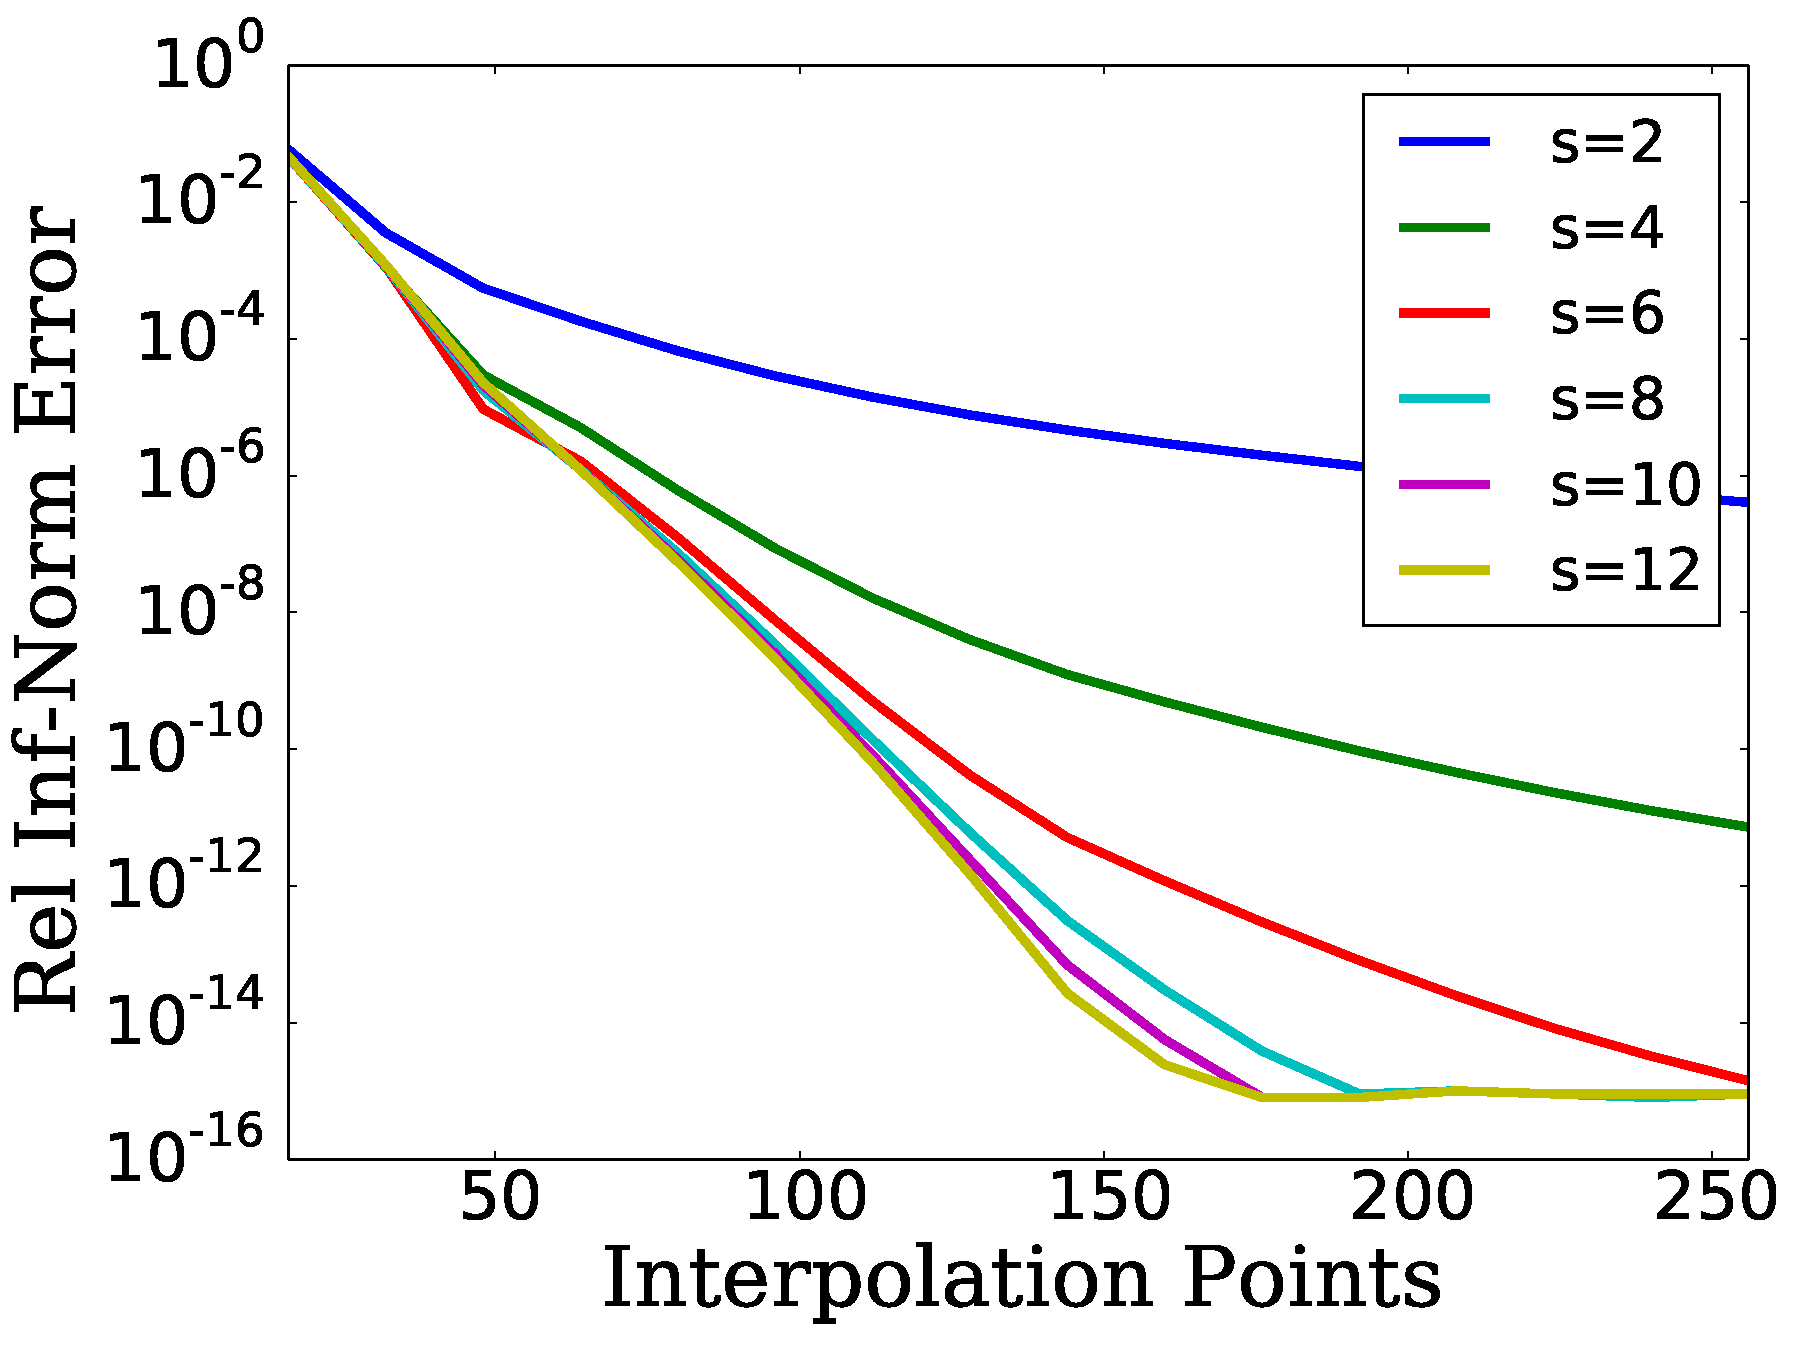
\includegraphics[width=\textwidth]{plots/msn_1d_smooth_R_25.pdf}
    \caption{$R=25$}
    \end{subfigure}
    \begin{subfigure}{0.45\textwidth}
    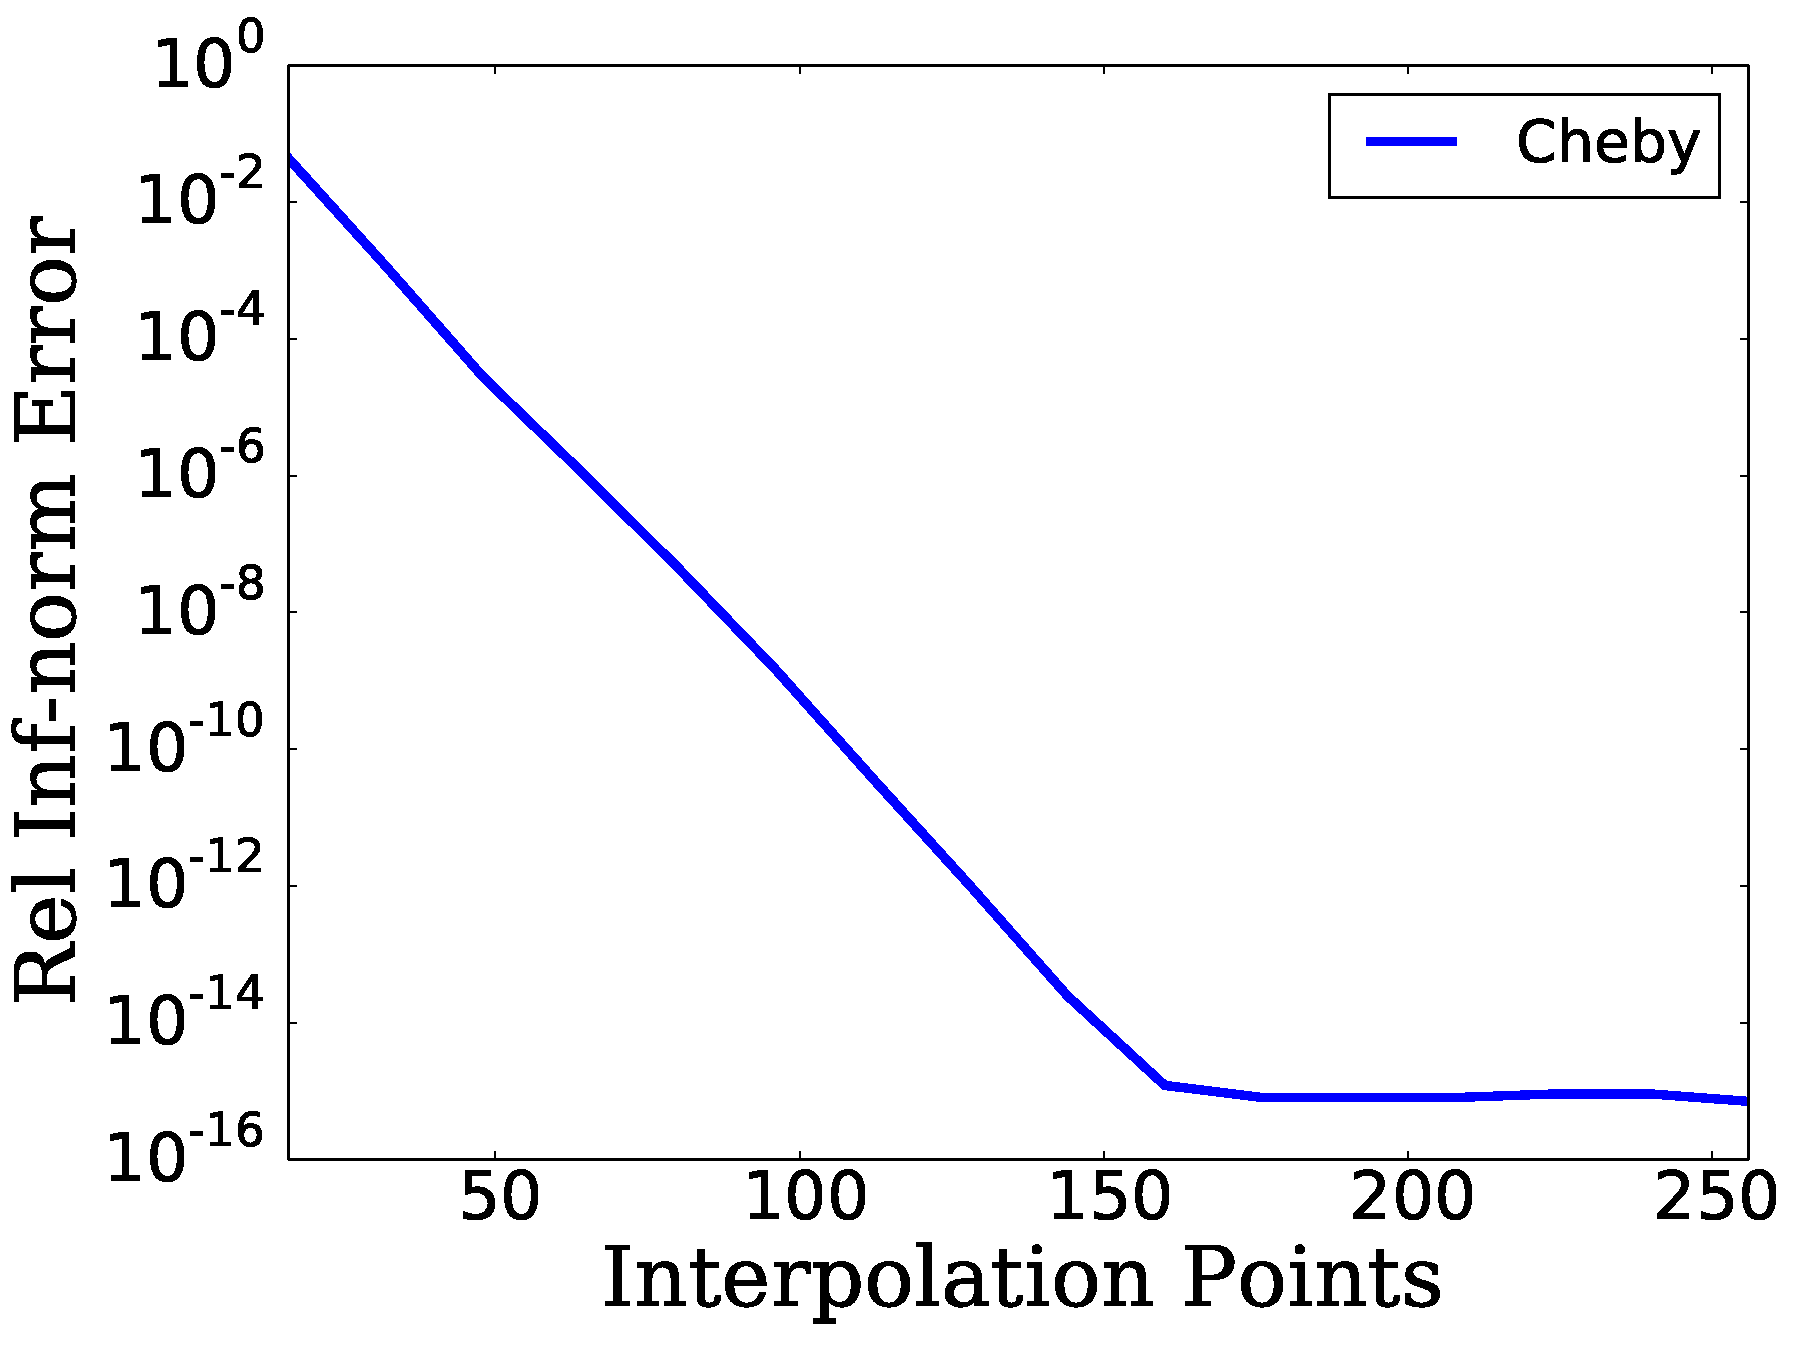
\includegraphics[width=\textwidth]{plots/cheby_1d_smooth_R_25.pdf}
    \caption{$R=25$}
    \end{subfigure}

    \begin{subfigure}{0.45\textwidth}
    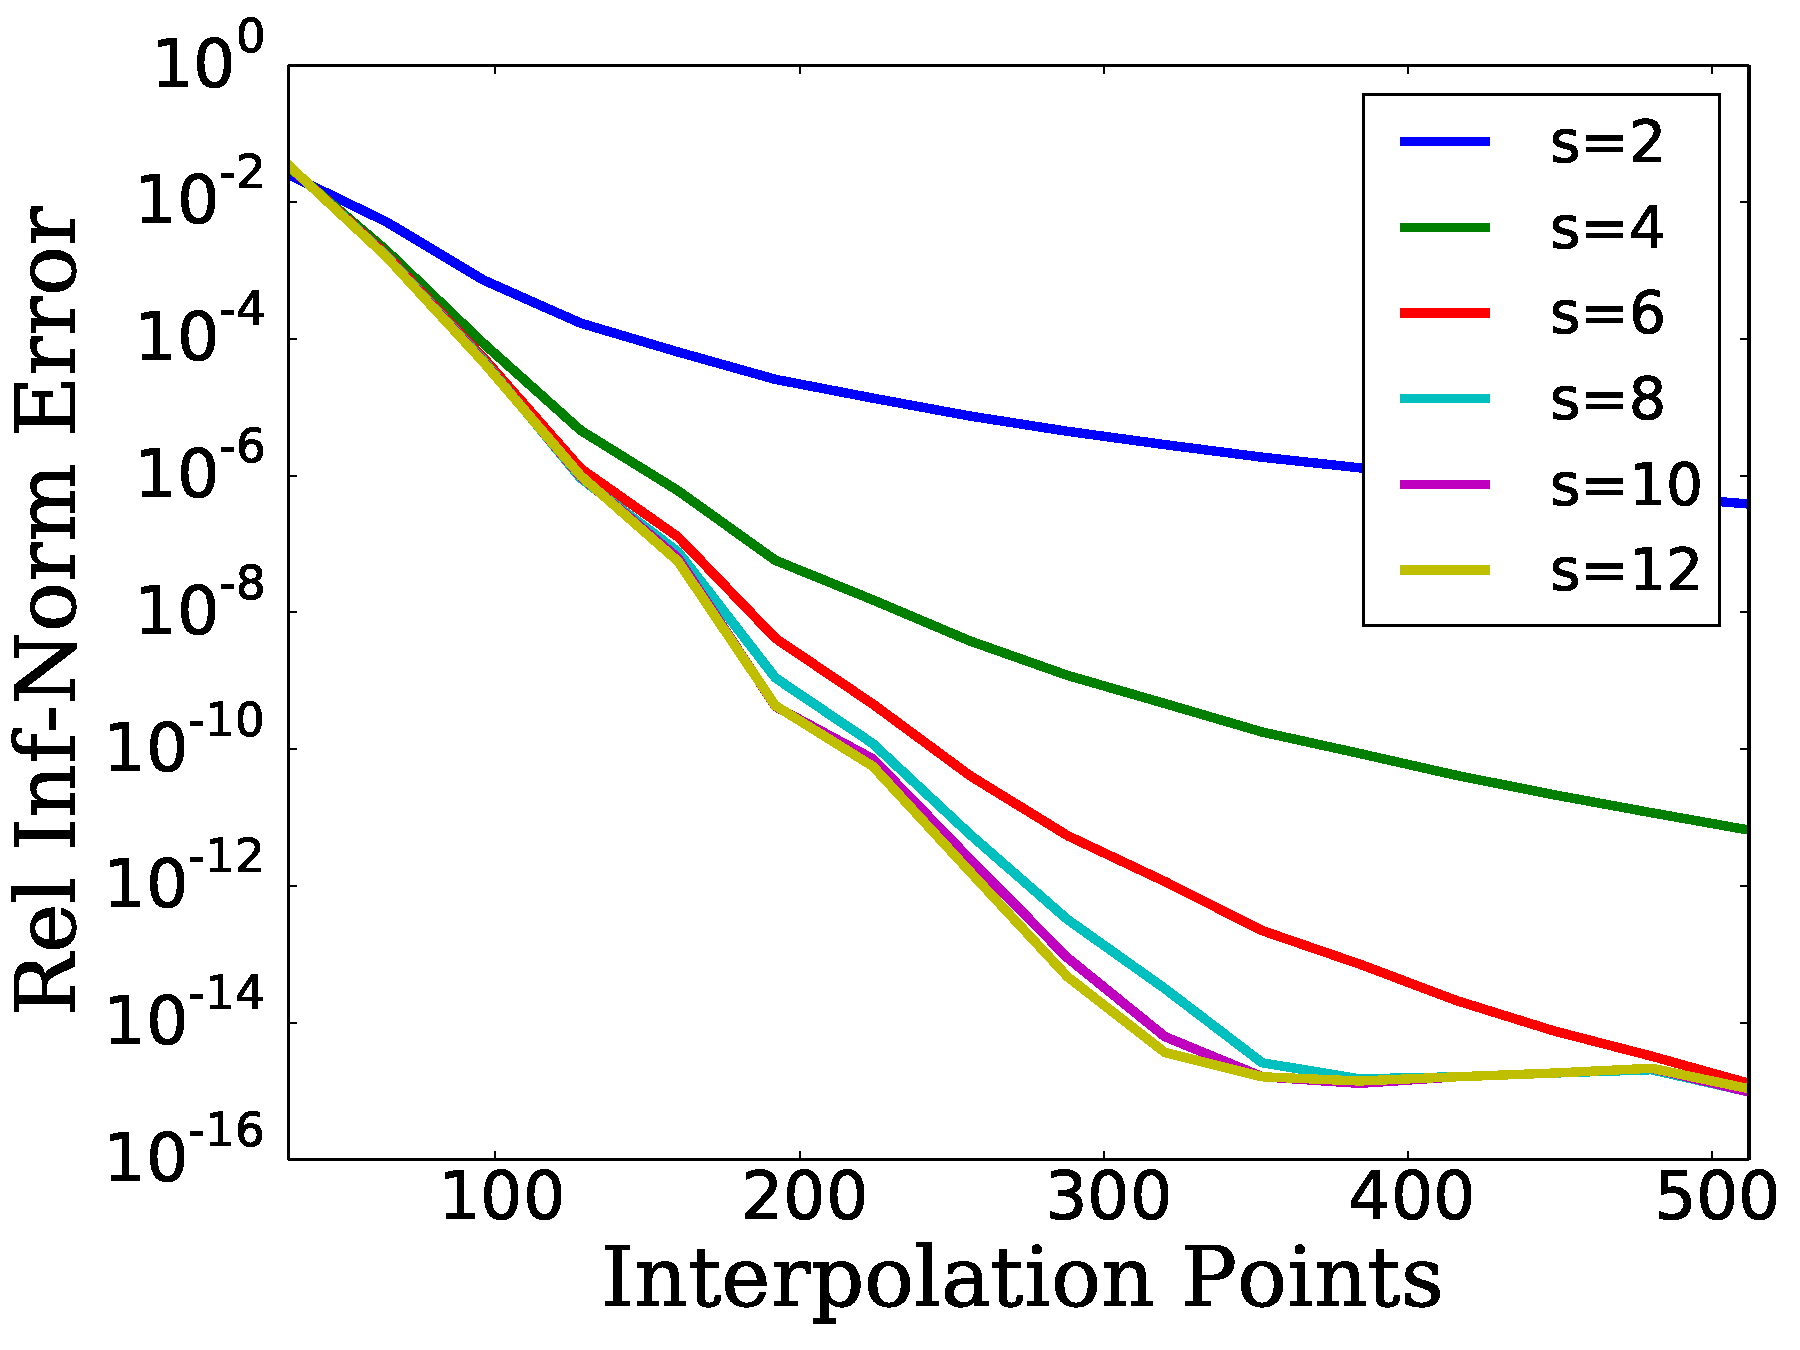
\includegraphics[width=\textwidth]{plots/msn_1d_smooth_R_100.pdf}
    \caption{$R=100$}
    \end{subfigure}
    \begin{subfigure}{0.45\textwidth}
    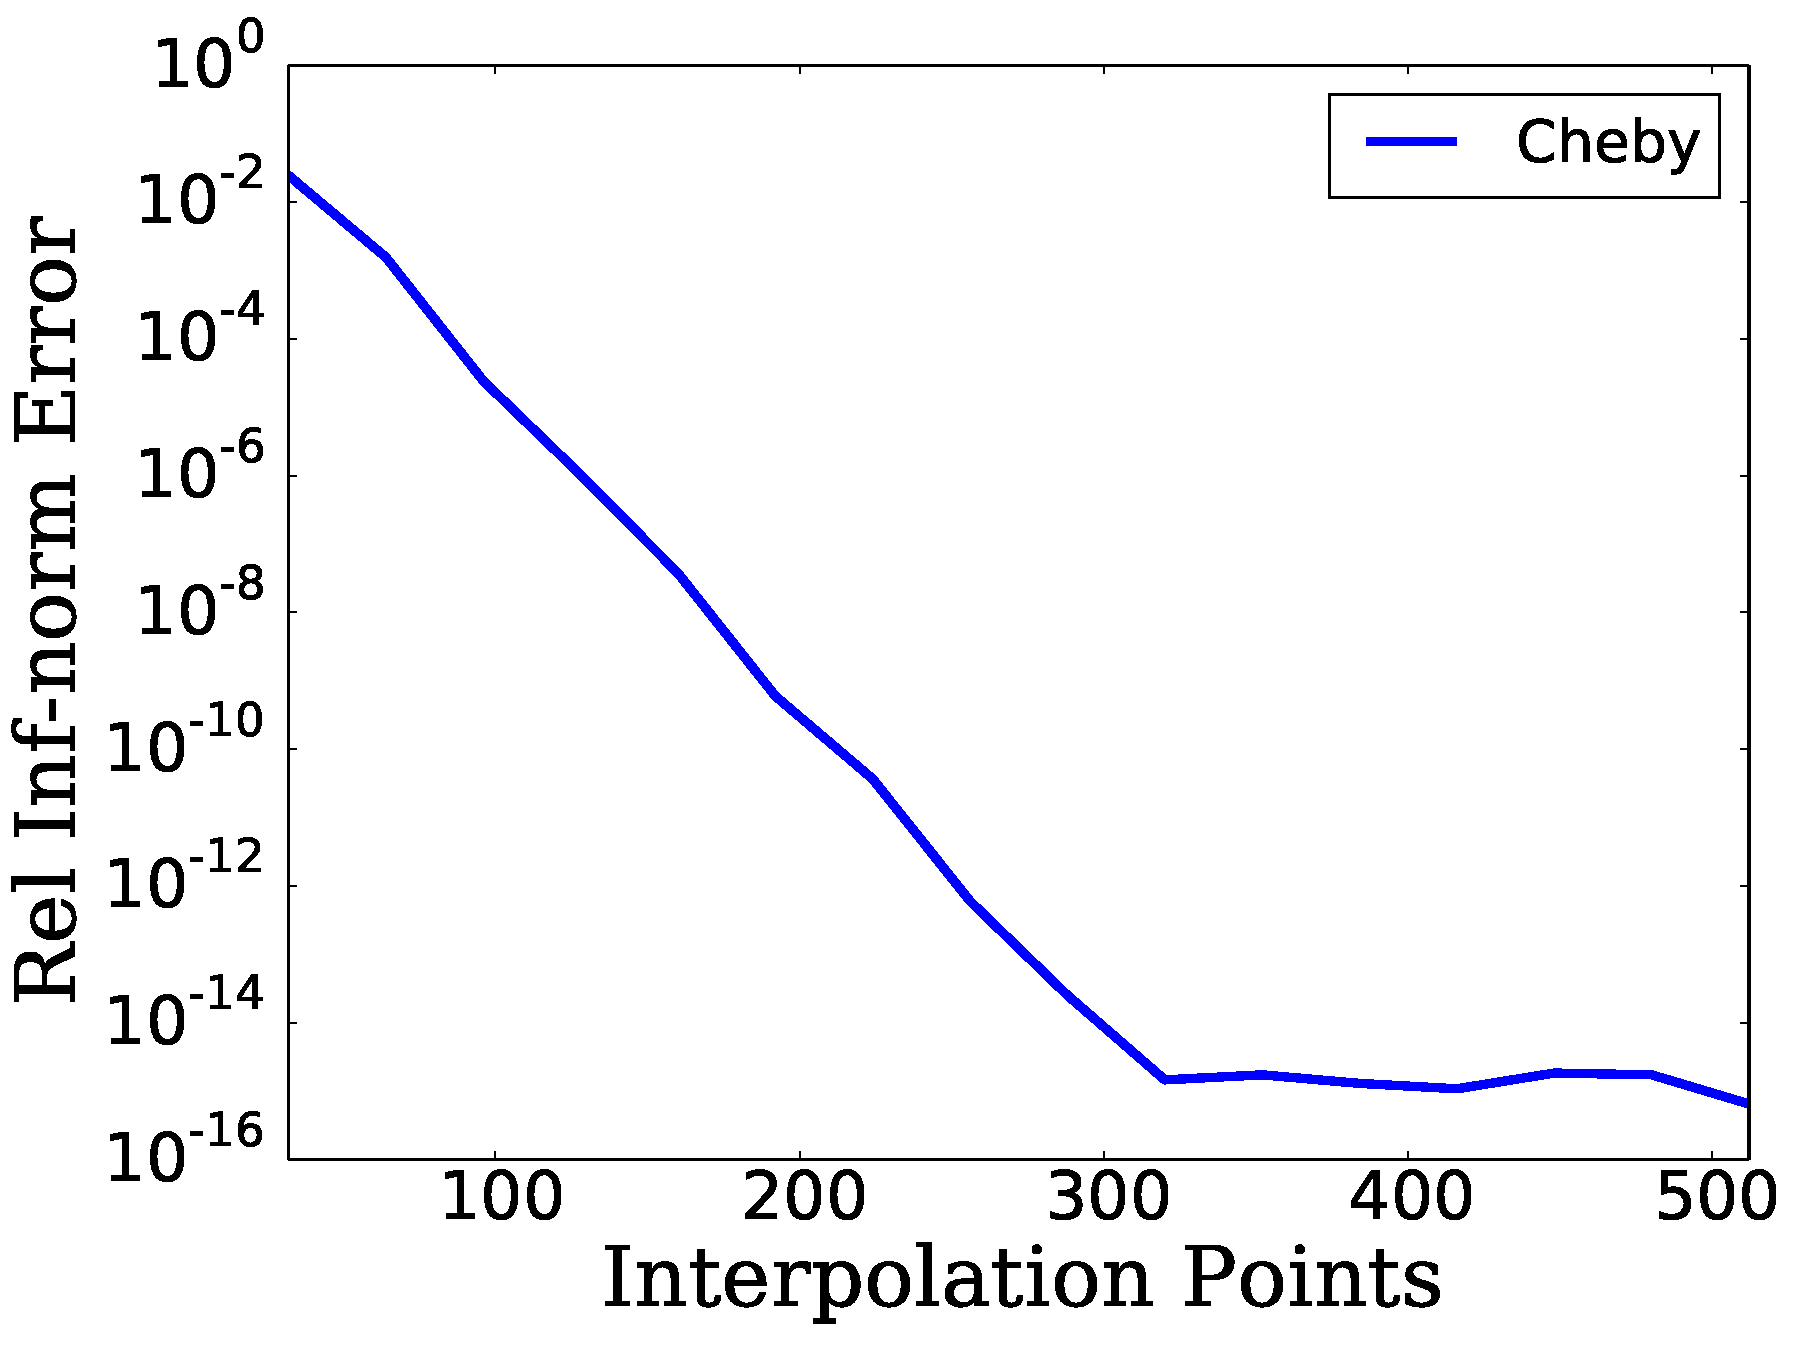
\includegraphics[width=\textwidth]{plots/cheby_1d_smooth_R_100.pdf}
    \caption{$R=100$}
    \end{subfigure}

\caption[Smooth Interpolation Comparison: 1D Runge Function]{
MSN interpolation and Chebyshev interpolation results of the
1D Runge function $g_{25}$ and $g_{100}$ for various $s$ values.
}
\label{fig:smooth_comparison_1d_runge}
\end{figure}





\subsection{Birkhoff Interpolation Comparison}

We now look at a Birkhoff interpolation problem for an approximation $p$:
%
\begin{align}
    p'(z_{k}^{n}) &= g_{R}'(z_{k}^{n}), \quad k\in\braces{1,\cdots,n}
        \nonumber\\
    p(-1) &= g_{R}(-1) \nonumber\\
    p(1) &= g_{R}(1).
\end{align}
%
Fast MSN methods exist and we compare against Chebyshev interpolation.
In particular, the system
%
\begin{equation}
    \begin{bmatrix} UWD \\ A \end{bmatrix} a
        = \begin{bmatrix} UC^{-1}f' \\ f \end{bmatrix},
    \label{eq:smooth_birkhoff_system}
\end{equation}
%
where $f'$ holds the derivative information and $f$ holds the
endpoint interpolation, is solved using pivoted QR.
The $UWD$ matrix is truncated so that the entire system is square,
and from our previous work we know $UWD$ is mostly zero.
The standard method for solving linear systems in Julia
is pivoted LU~\cite{julialang}, although there is no noticeable difference
between pivoted QR and pivoted LU (results not shown).
The results for can be seen in
Fig.~\ref{fig:smooth_comparison_1d_runge_birkhoff}.
When solving the square system, it is clear numerical
difficulties are keeping the minimal error around $10^{-14}$.
The error decay of both methods are approximately the same.

Due to the structure of the linear system, it would be possible
to implement a similar fast solver for the square system.

% Print results for comparing MSN with 2D Runge function

\begin{figure}[p]
    \centering
    \begin{subfigure}{0.45\textwidth}
    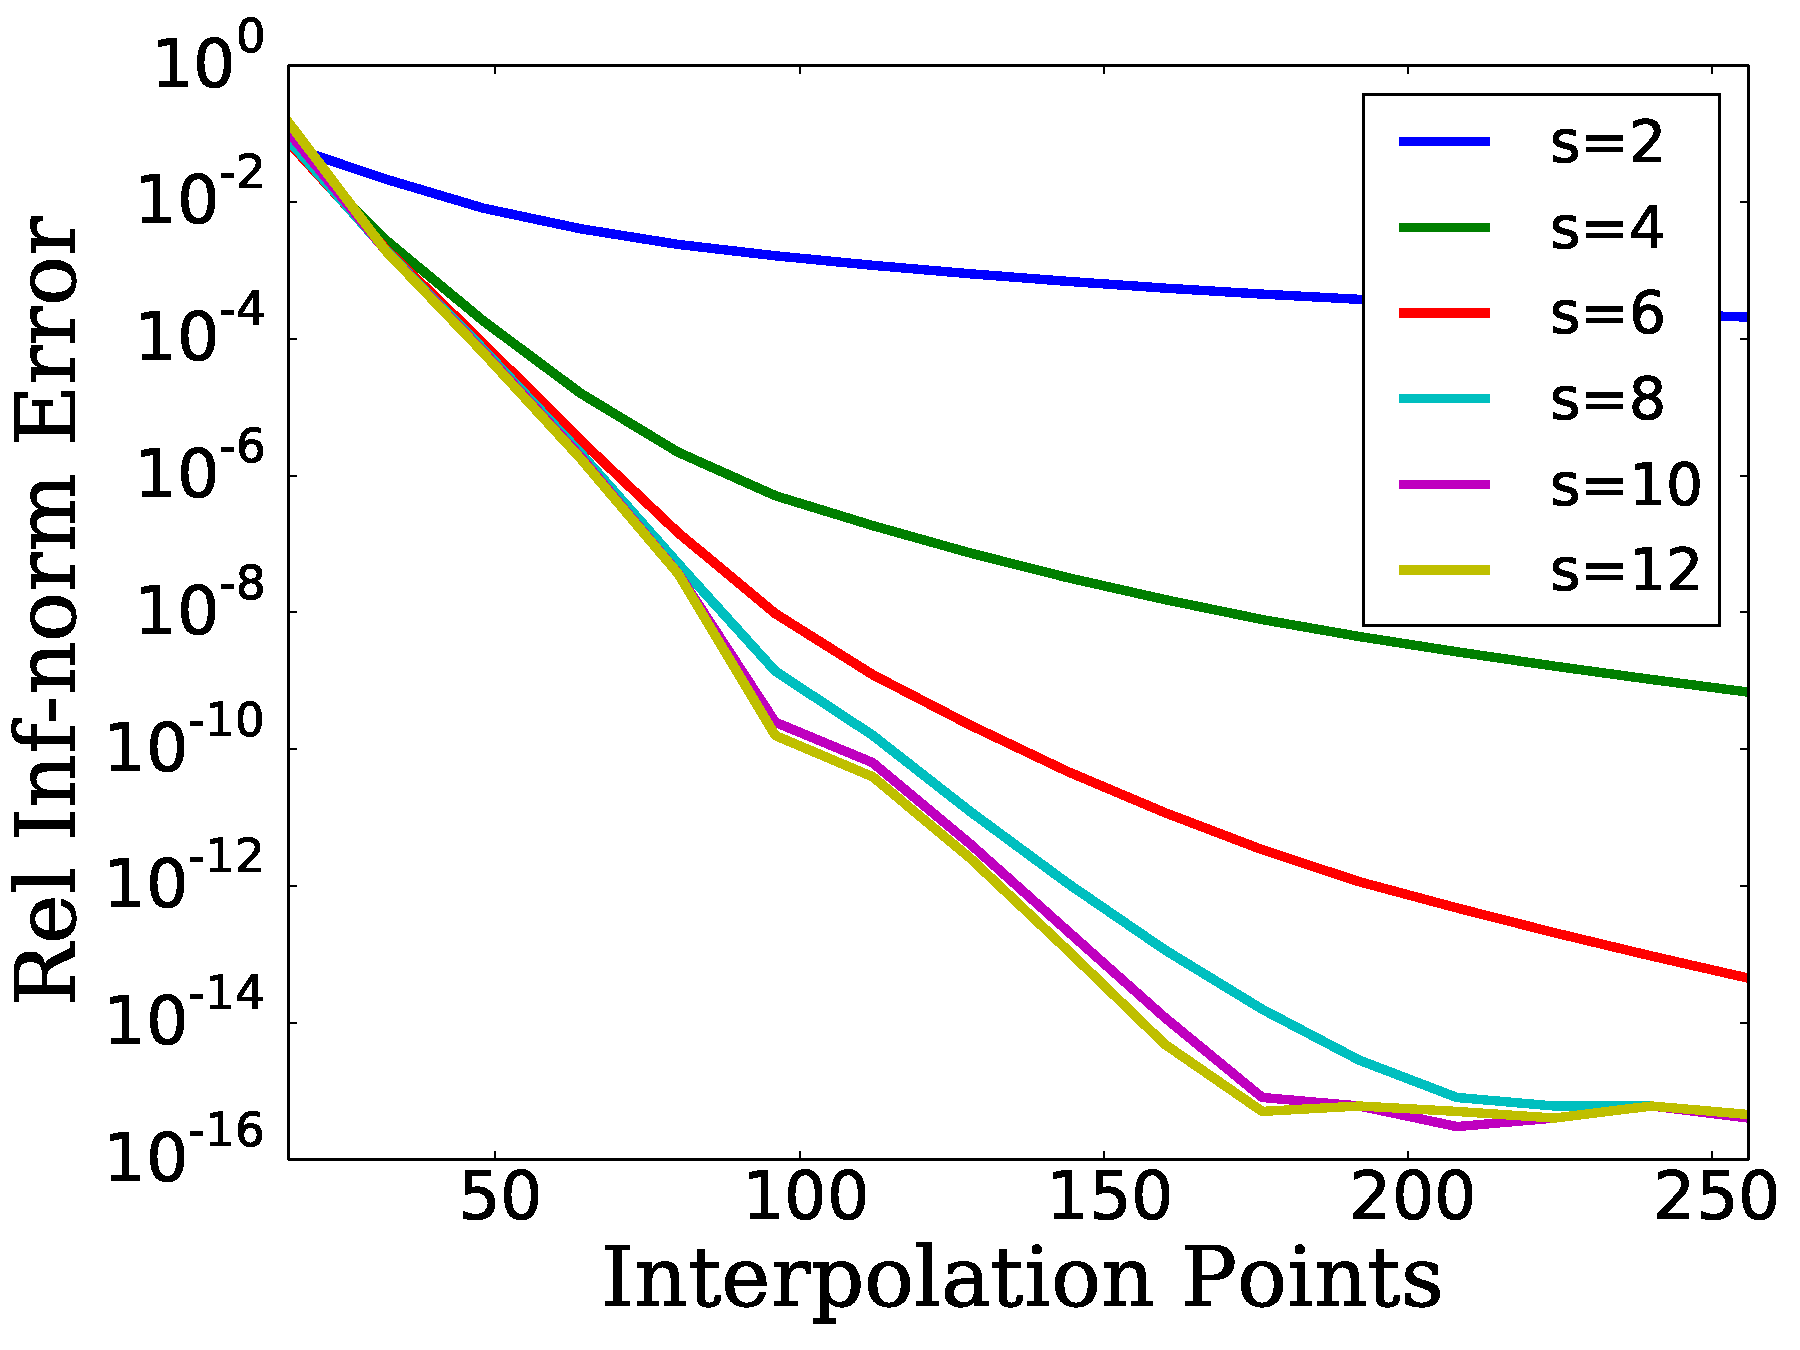
\includegraphics[width=\textwidth]{plots/msn_1d_birkhoff_smooth_R_25.pdf}
    \caption{$R=25$}
    \end{subfigure}
    \begin{subfigure}{0.45\textwidth}
    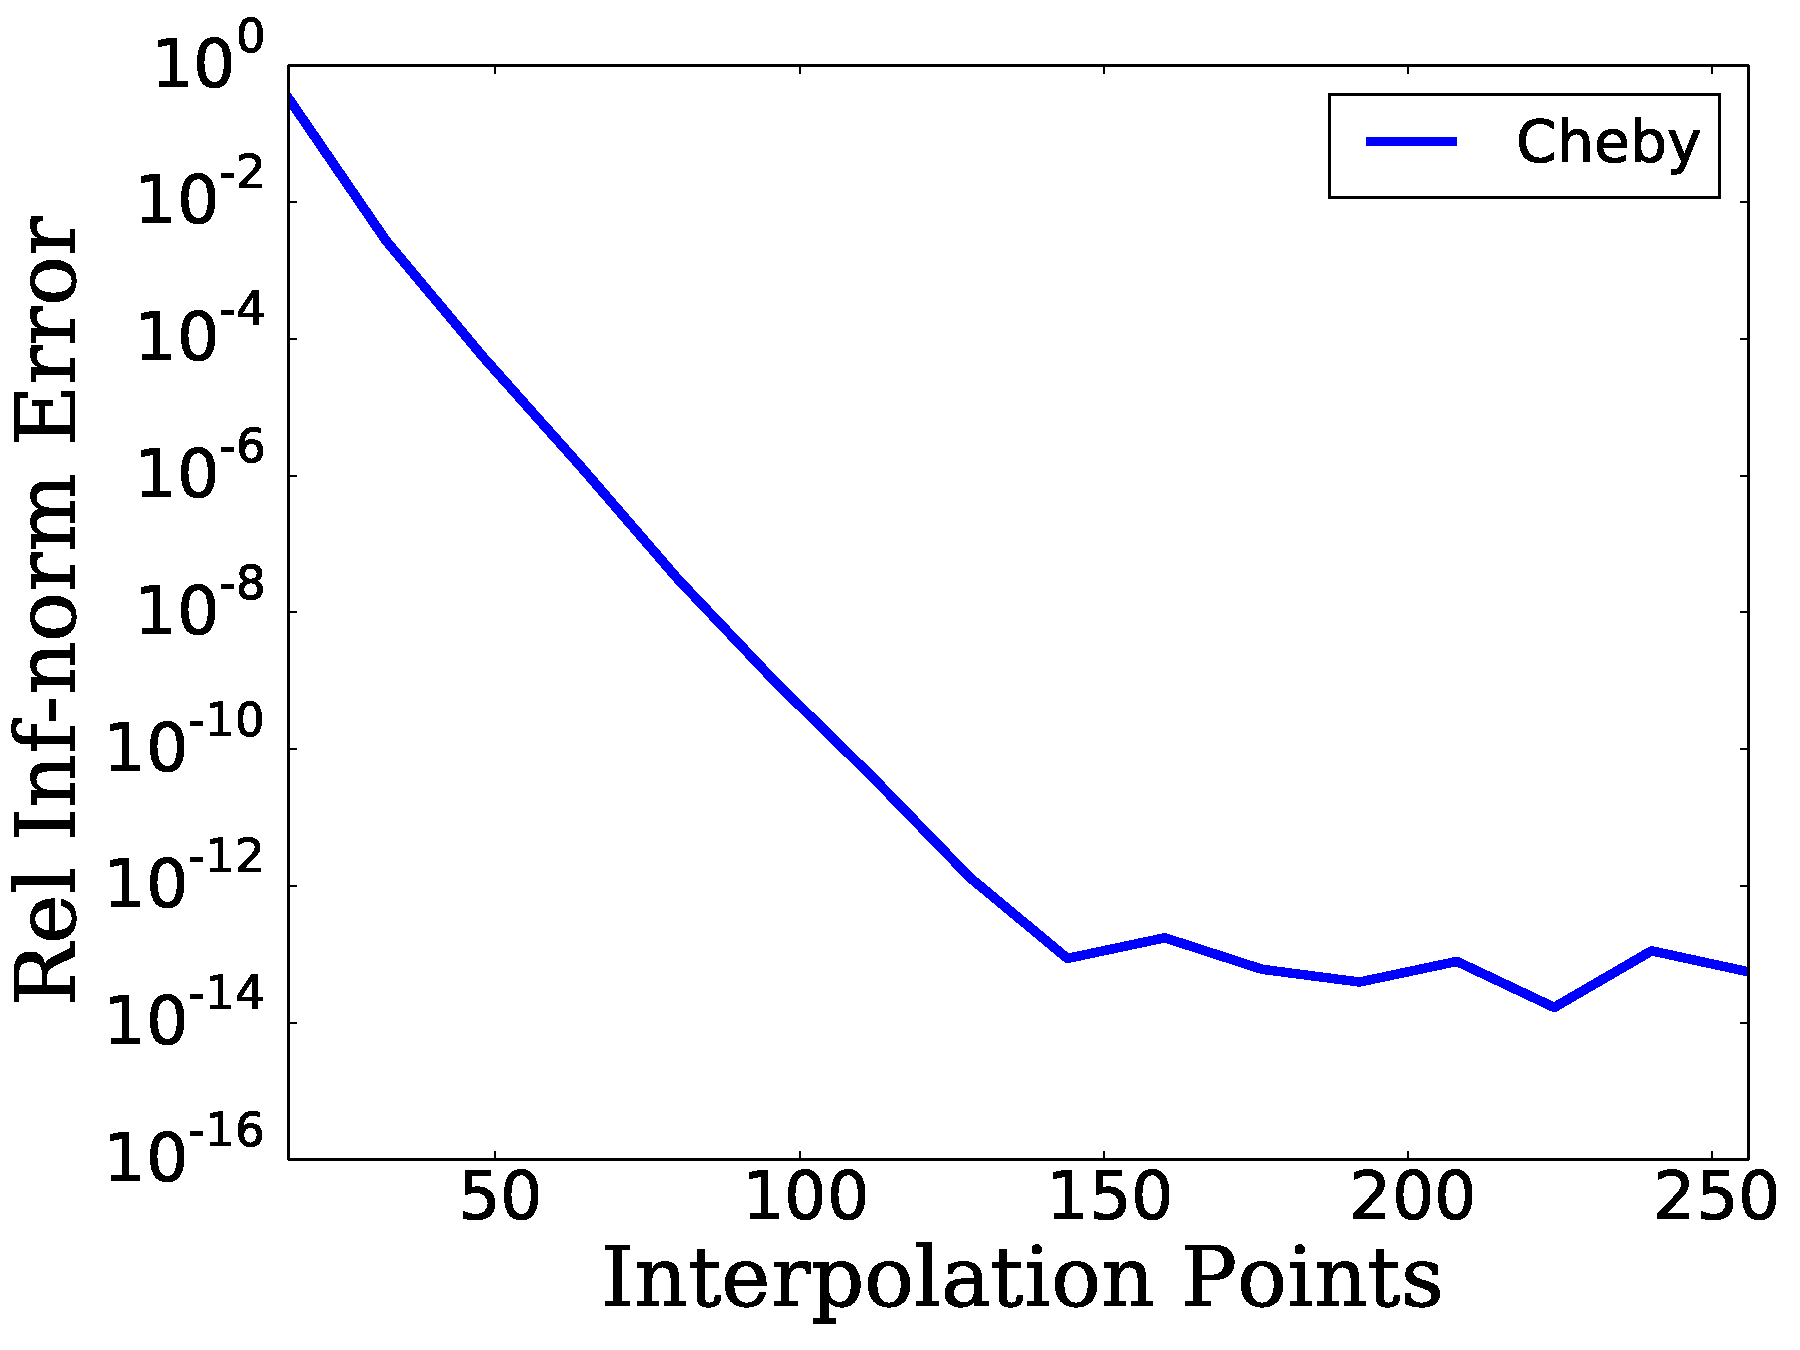
\includegraphics[width=\textwidth]{plots/cheby_1d_birkhoff_smooth_R_25.pdf}
    \caption{$R=25$}
    \end{subfigure}

    \begin{subfigure}{0.45\textwidth}
    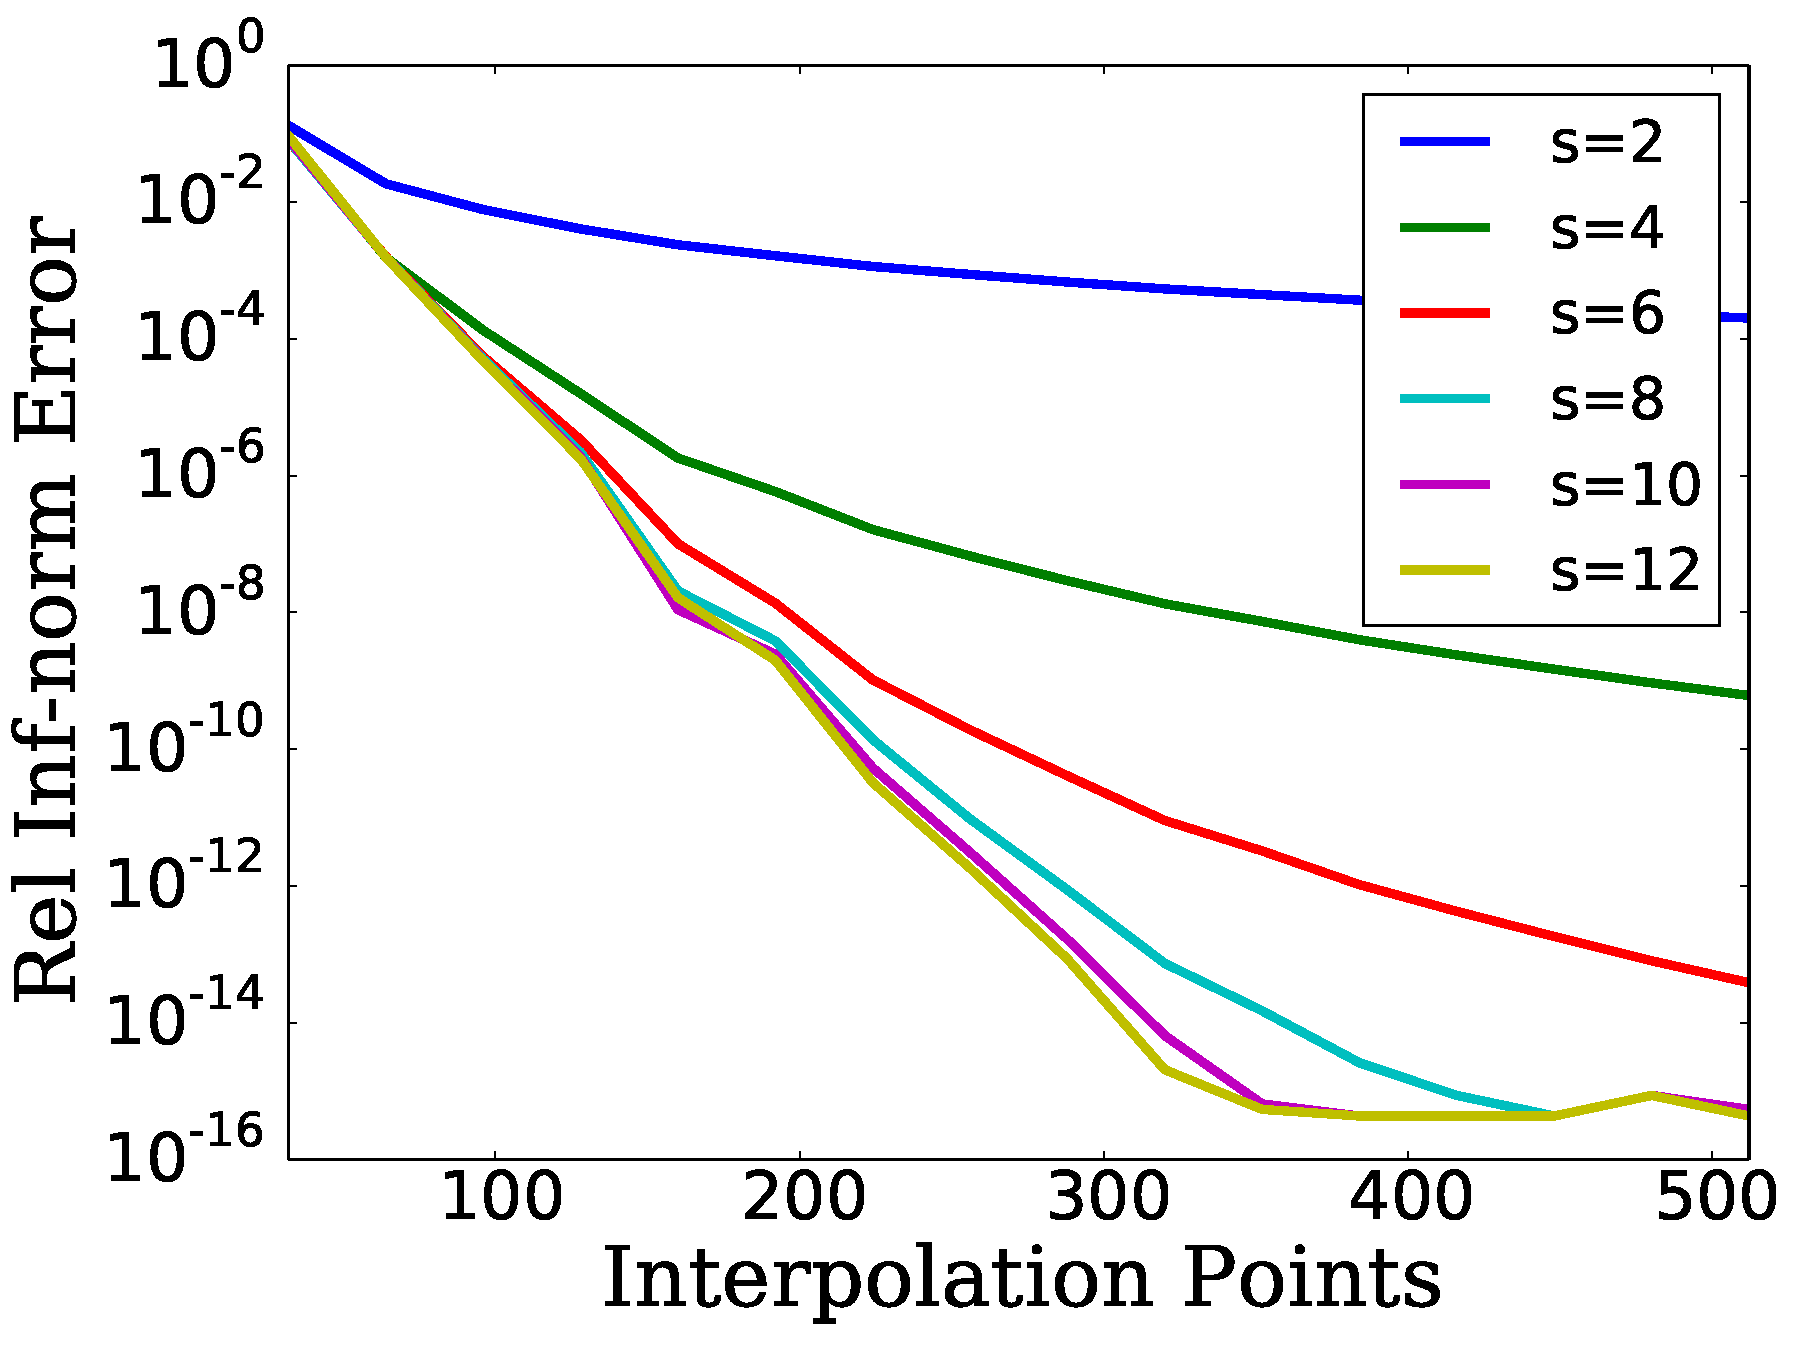
\includegraphics[width=\textwidth]{plots/msn_1d_birkhoff_smooth_R_100.pdf}
    \caption{$R=100$}
    \end{subfigure}
    \begin{subfigure}{0.45\textwidth}
    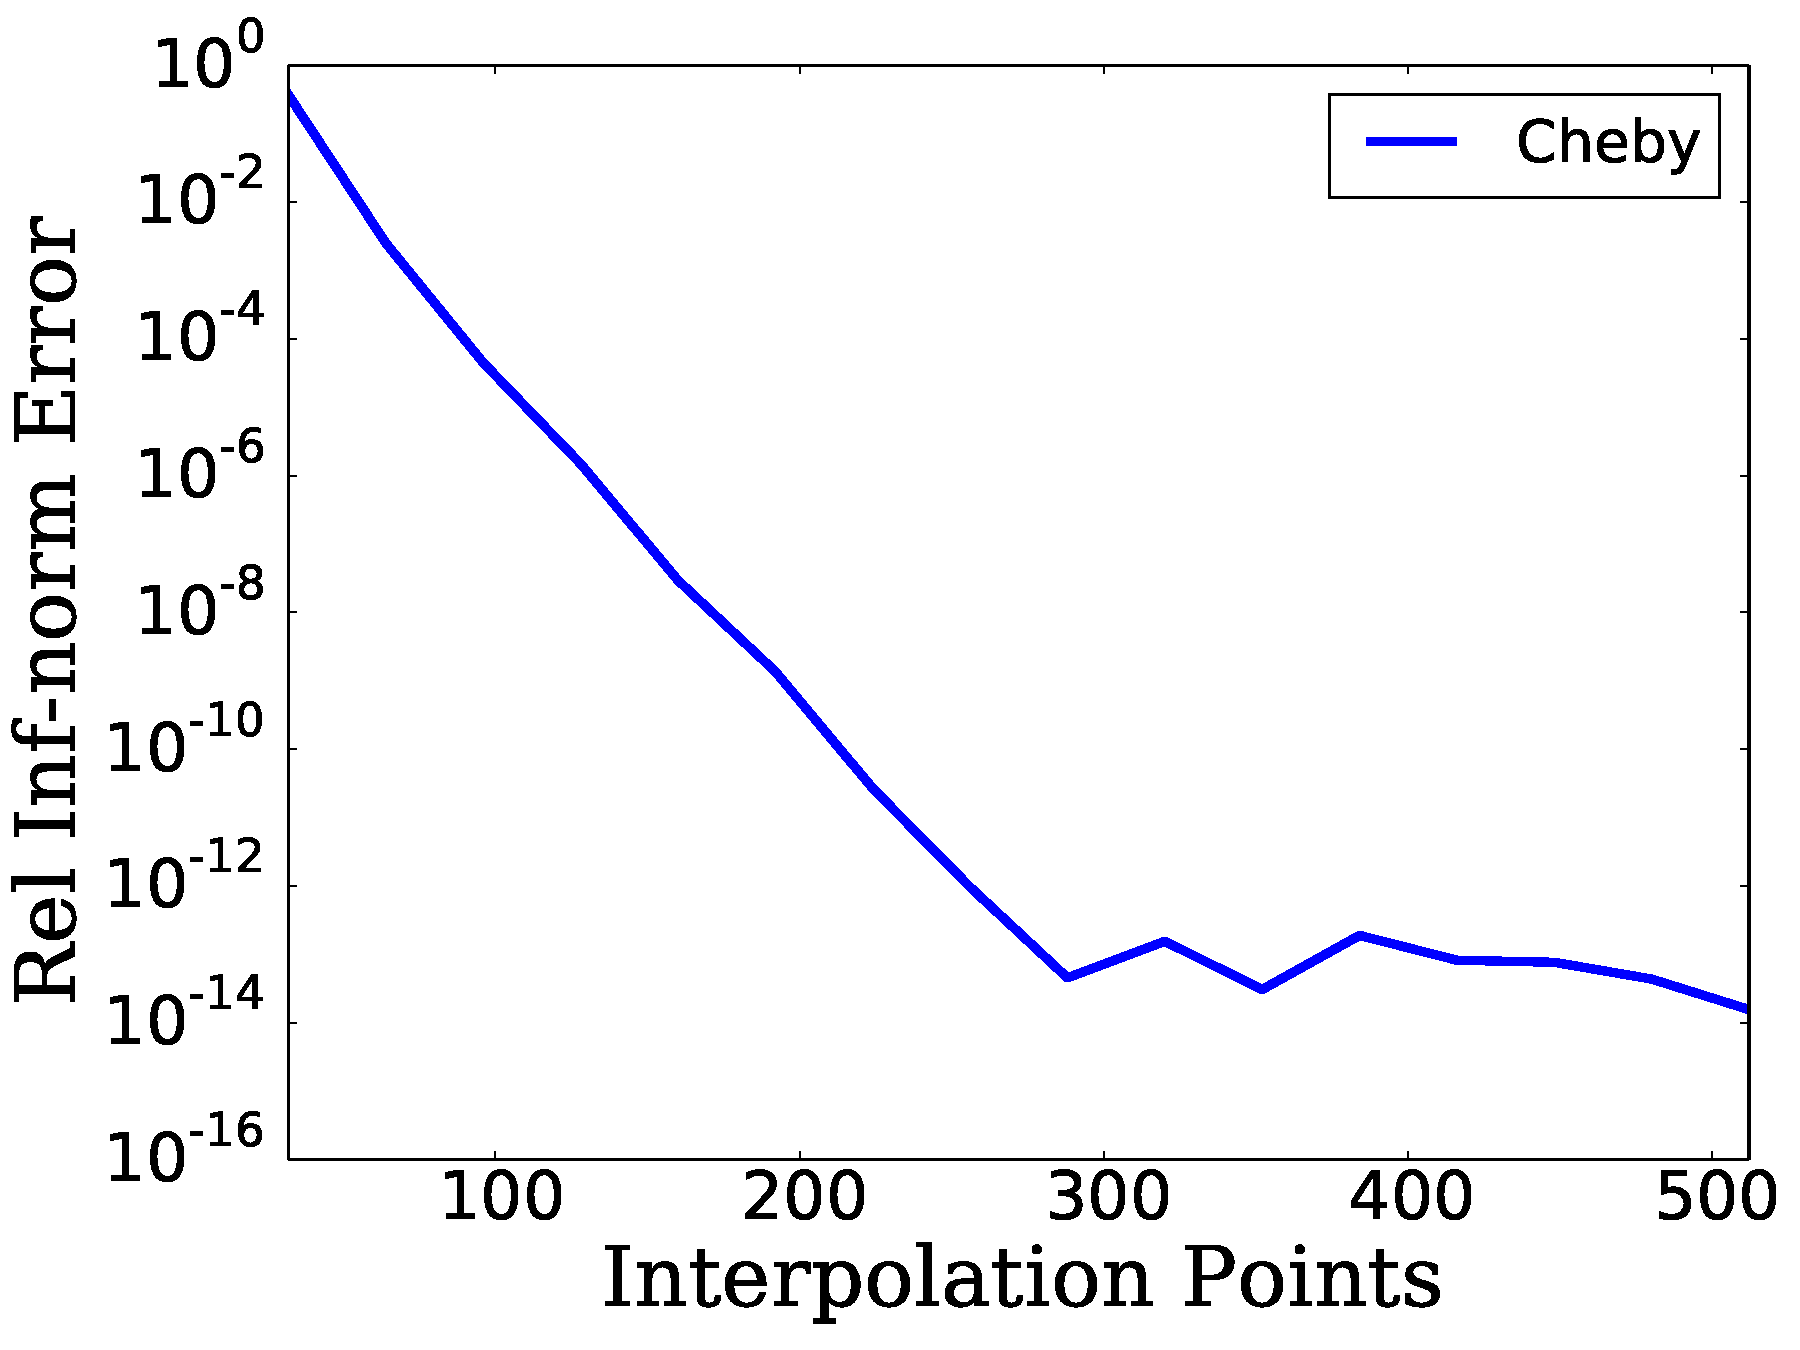
\includegraphics[width=\textwidth]{plots/cheby_1d_birkhoff_smooth_R_100.pdf}
    \caption{$R=100$}
    \end{subfigure}

\caption[Smooth Birkhoff Interpolation Comparison: 1D Runge Function]{
MSN Birkhoff interpolation and Chebyshev interpolation results
of the 1D Runge function $g_{25}$ and $g_{100}$ for various $s$ values.
}
\label{fig:smooth_comparison_1d_runge_birkhoff}
\end{figure}




